\chapter{Architectural Design}

\section{Overview}

\begin{figure}[H]
	\centering
	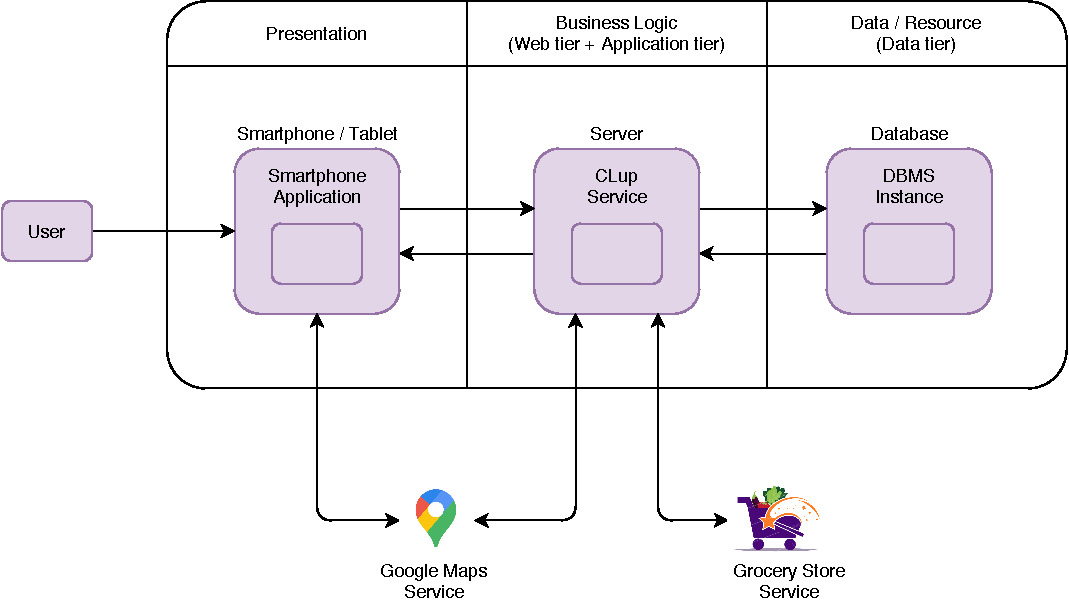
\includegraphics[width=1.0\textwidth]{images/architecture.pdf}
	\caption{System architecture.}
\end{figure}

\section{Component View}

The previously introduced components will be presented in details in this section by using the component diagram~\ref{fig:ComponentDiagram} that has been divided in three main sub-components to better understand the relation between the three tiers of the system.

The presentation tier has been represented by the \textbf{EndUserApp} that generalizes the architecture of the smartphone application.
It encapsulates the \textbf{\gls{mvc}}, that has been chosen as design pattern, and the \textbf{HostService} which is the module that allows the application to use the \glspl{api} offered by the device.

\begin{sidewaystable} % \begin{figure}[H]
	\centering
	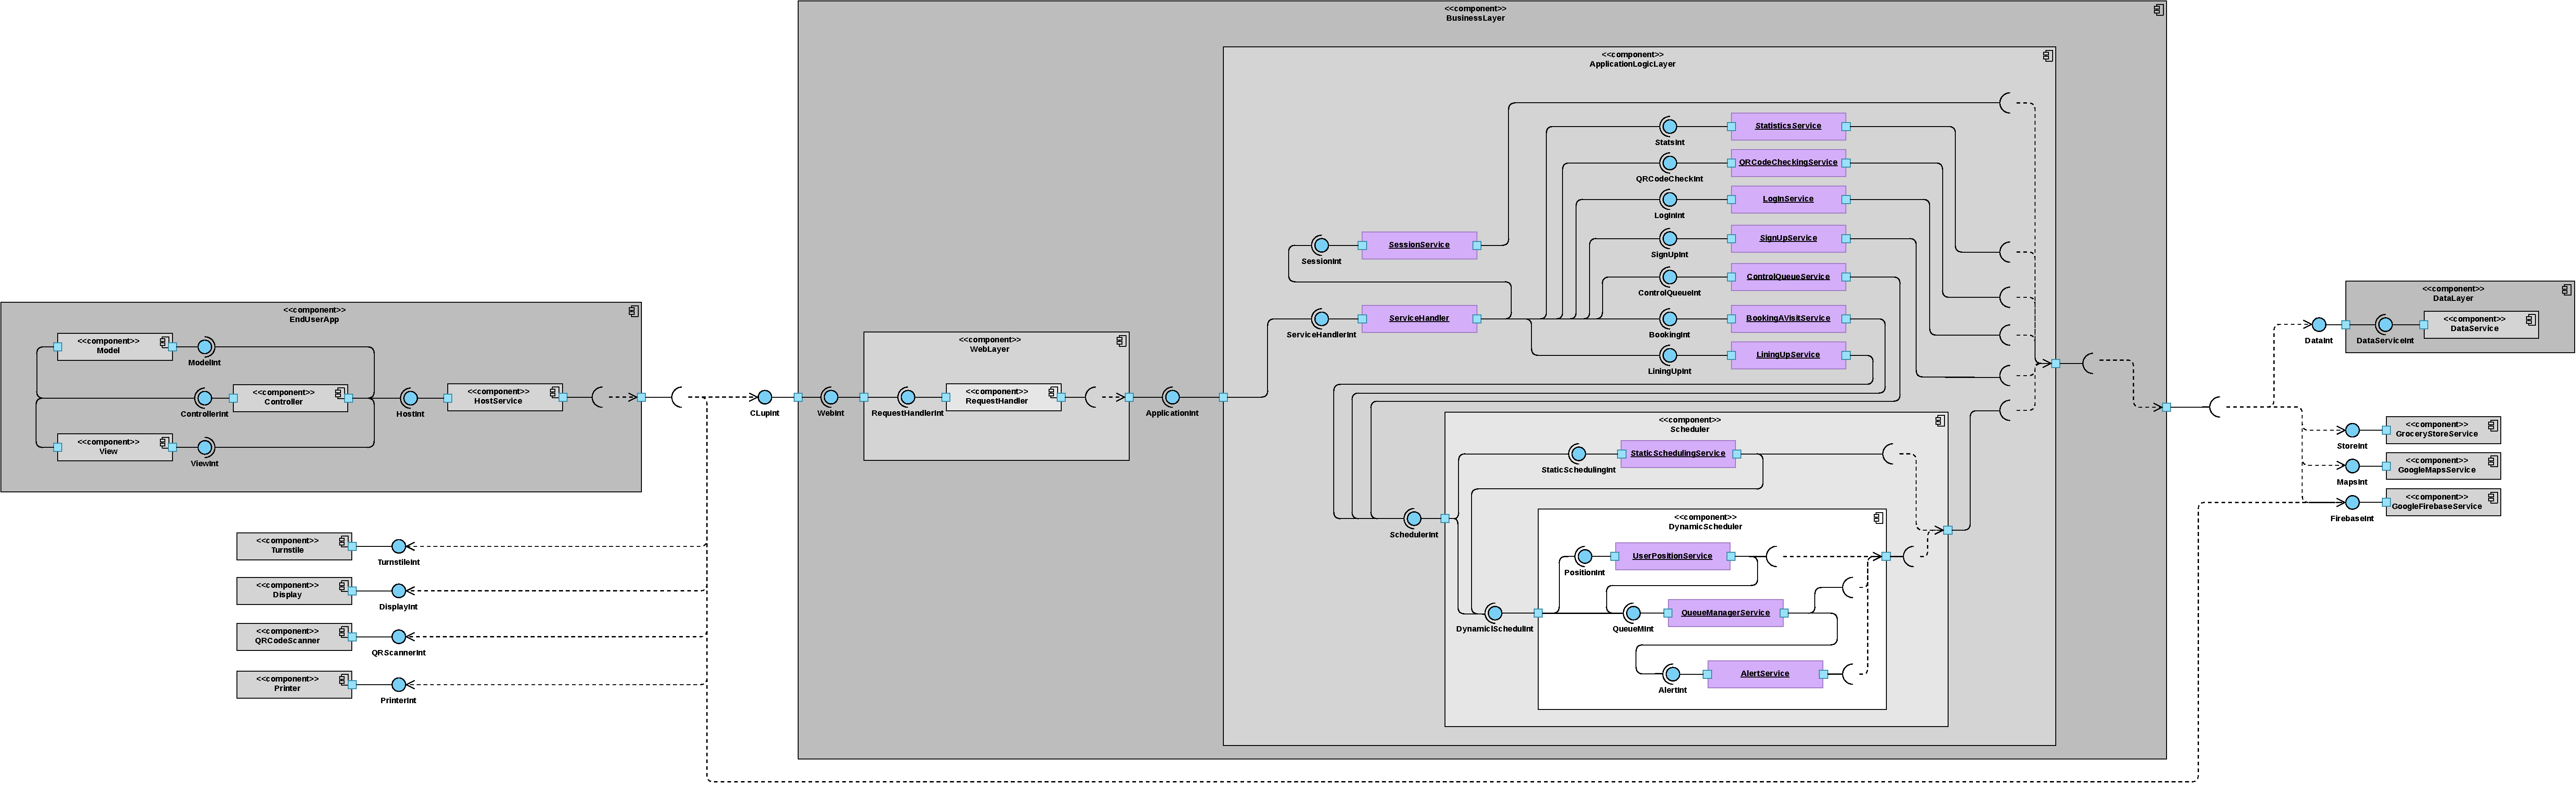
\includegraphics[width=1.0\textwidth]{images/component_diagram.pdf}
	\caption{Component Diagram.}\label{fig:ComponentDiagram}
\end{sidewaystable} % \end{figure}

The business tier (web tier \& application tier) is the most complex part of the diagram, therefore it has been split in different layers of components:
\begin{itemize}
	\item \textbf{WebLayer}: contains the \textbf{RequestHandler} component that receives the requests from remote devices and forwards them to the application tier. The main functionalities are: \textit{decryption}, \textit{parsing} and \textit{forwarding} of the requests; \textit{reformatting} (in \gls{json} format) and \textit{encryption} of the responses before sending them to the clients.
	
	\item \textbf{ApplicationLogicLayer}: contains the modules for the functionalities offered by the system. They are:
		\begin{itemize}
			\item \textbf{ServiceHandler}: is the module that coordinates the others. It receives the requests from the previous layer and checks if sessions are active, communicating with the SessionService. After that, it calls the other services based on the request type. In the end, it returns the responses to the WebLayer.
			\item \textbf{SessionService}: is the service that monitors the session by updating and releasing tokens.
			\item \textbf{StatisticsService}: is the service that creates charts for the store manager to analyze the trend of the queues. It interacts with the DataLayer to retrieve data from the database.
			\item \textbf{QRCodeCheckingService}: is the service used when customers scan the QR codes to verify that the ticket numbers are the same that have been notified by the system. It is called, in background, by the application running on the store manager device.
			\item \textbf{LogInService}: is the service that controls and updates the status of the tokens. If an user has been recognized, by the system, it changes the status of the token in the database. In this way, the user will be identified as logged and he will be able to request for services that requires an authentication.
			This service is used for log out too.
			\item \textbf{SignUpSerivice}: allows users to create an account.
			\item \textbf{ControlQueueService}: is the service used by the store manager to change parameters that modify the sequence of events in the Scheduler. From this service the store manager can modify the timing in which tickets are released, he can interrupt the release of tickets and he can change other parameters of the scheduler algorithm. This service communicates with the Scheduler and the DataLayer to store the new parameters.
			\item \textbf{BookingAVisitService}: is the service that allows customers to book a visit. It handles the data passed from the clients, performs some checks on the inserted information and communicates with the Scheduler and with the DataLayer.
			\item \textbf{LiningUpService}: is the service that allows customers to line up. As for the BookingAVisitService, it passes data to the Scheduler and the DataLayer.
		\end{itemize}
		
		The main core of the ApplicationLogicLayer is the \textbf{Scheduler} that implements the algorithm used by the system to create and keep updated the virtual queue of users. It is composed by a StaticSchedulingService and a DynamicScheduler.
		\item The \textbf{StaticSchedulingService} is in charge of performing few checks before asking to the DynamicScheduler to insert customers in the queue. Moreover, it is the first sub-module to be called by the LiningUpService and the BookingAVisitService. It communicates with the external services to compute a raw estimation of the time in which a customer will be called by the system to be authorized to enter in the store.
		\item The \textbf{DynamicScheduler} is composed by different sub-services that are necessary to update the virtual queue in background and to notify customers.
		The main sub-service is the \textbf{QueueManagerService} that handles the queue and coordinates the other modules.
\end{itemize}

The data tier has been represented by the \textbf{DataLayer} that contains the \textbf{DataService}. It interacts with the \gls{dbms} to execute queries.

In the diagram has been reported the external services used by the system:
\begin{itemize}
	\item \textbf{GroceryStoreService}: to obtain data about customers from the store.
	\item \textbf{GoogleMapsService}: used to compute the estimated time to arrive to the store from the location of the customer.
	\item \textbf{GoogleFirebaseService}: used to notify customers.
\end{itemize}


\section{Deployment View}

\section{Runtime View}

In this section we are going to present how the components interact at runtime.

\subsection{Session Control}

The figure \footnote{For all the sequence diagrams, a custom notation has been used to show the input parameters of the methods (**data). It follows a programming language notation to represent inputs in a more compact way. In Python style, it can be interpreted as a dictionary data structure.}~\ref{fig:SessControl} shows the sequence diagram associated to the operations performed by the SessionService module to generate and to control the validity of a given token. The tokens are part of the request parameters, they are used to keep sessions alive with users. The SessionService checks if a token already exists; if it is, then the module controls if it is valid or expired, otherwise it will generate a new one.
Authentications and tokens are two different things: an user can have a token but he might be unauthorized (not logged or he could not have an account yet). The authorization status, associated to a token, will be updated by the LogInService or by activities performed in background by the system.

\begin{figure}[H]
	\centering
	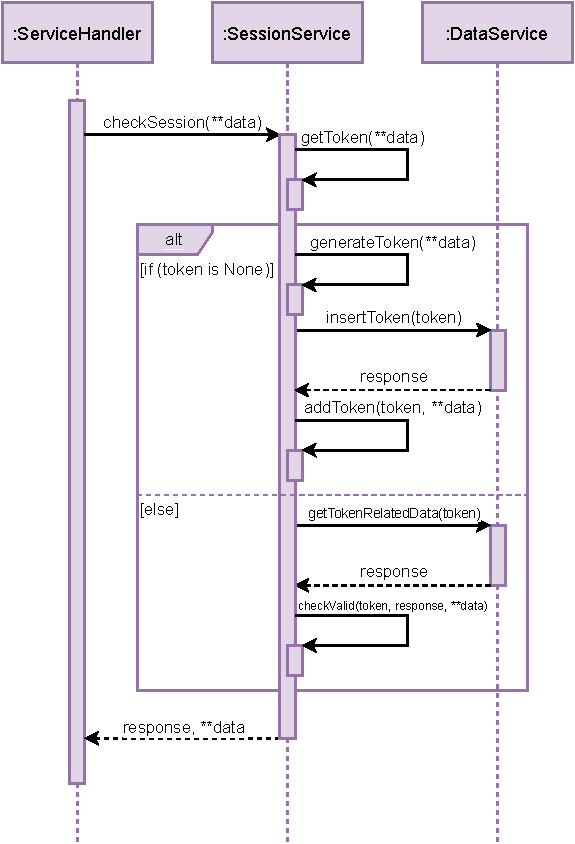
\includegraphics[width=1.0\textwidth]{images/sessionToken_sequence_diagram.pdf}
	\caption{Session control sequence diagram.}\label{fig:SessControl}
\end{figure}

\subsection{Sign Up}

In figure~\ref{fig:SignUp} has been shown the procedure to register a new user. The core of the sequence diagram is the SignUpService that filters the data inserted by the customers and controls if the credentials have already been used for other accounts. If possible, the service creates the new account by inserting the credentials, and the other customers information, in the database. Results of the queries and the other executed methods are appended to the data that are back-propagated to the RequestHandler that creates the \gls{json} response.

\begin{figure}[H]
	\centering
	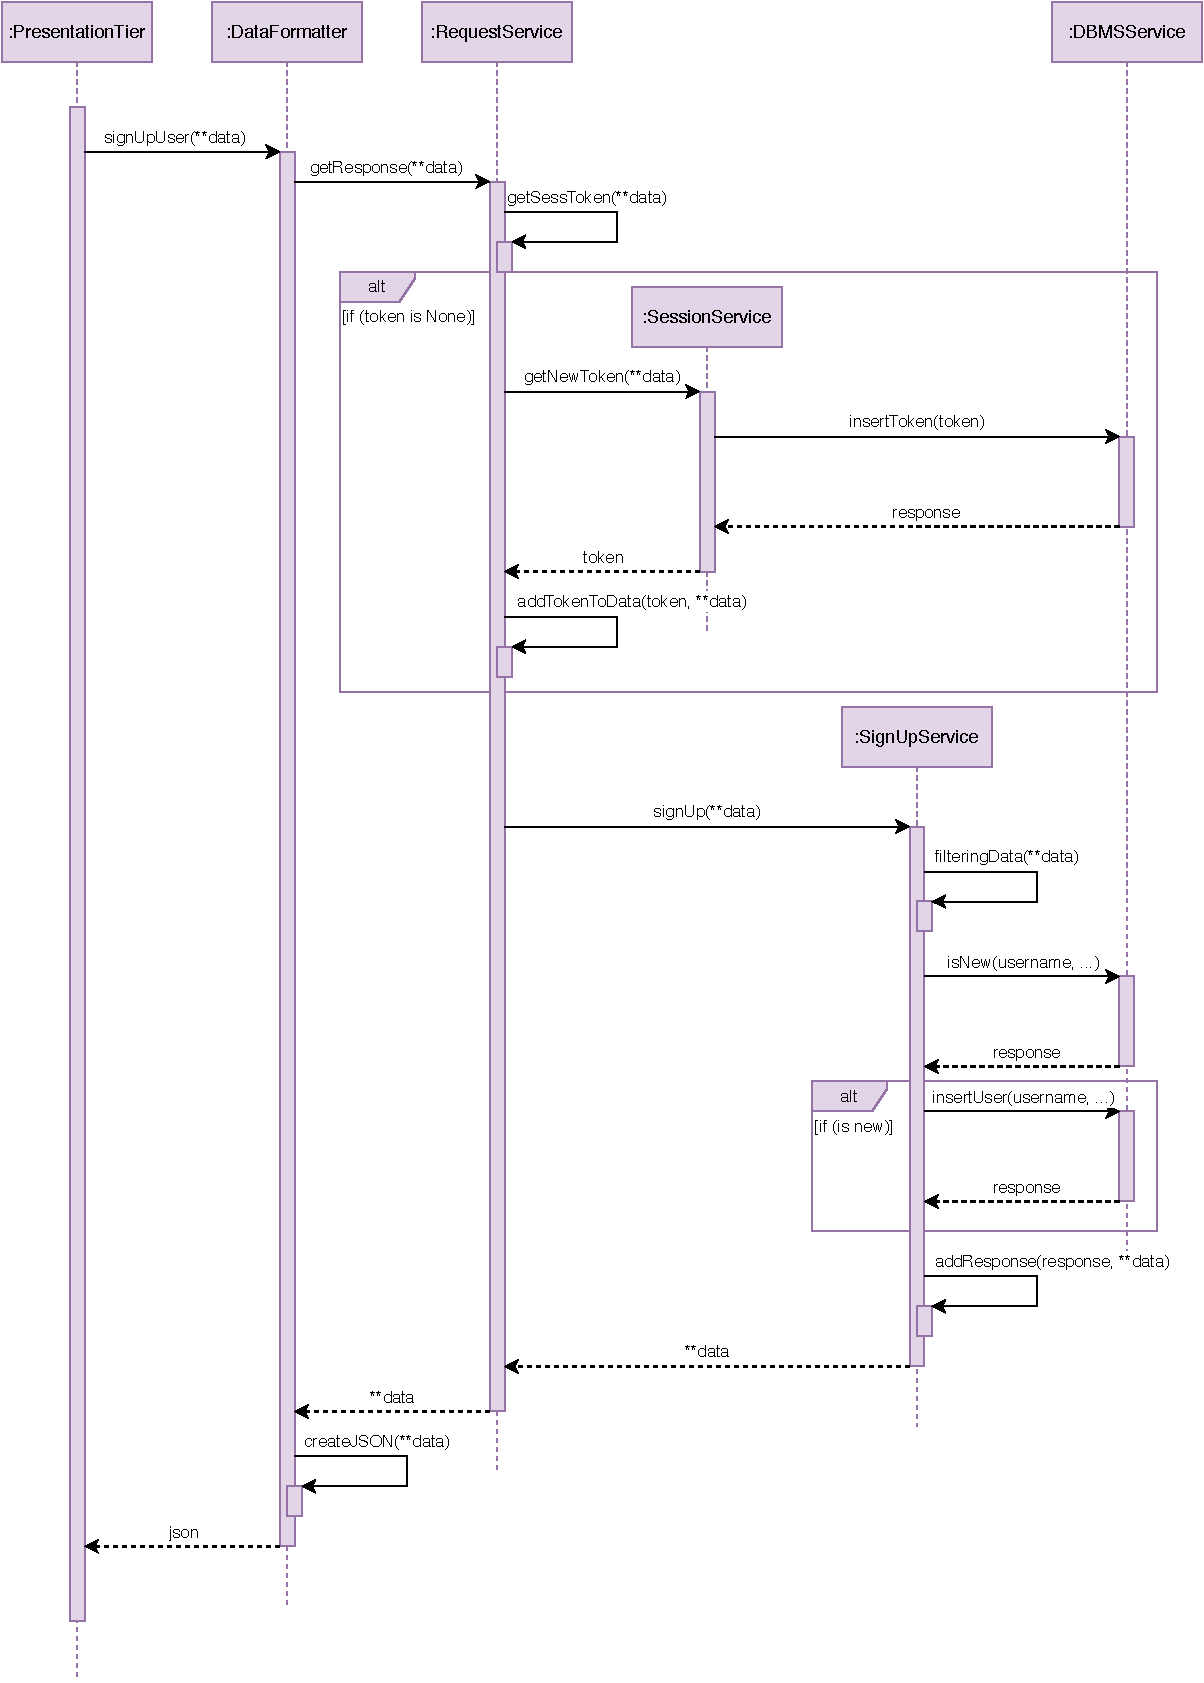
\includegraphics[width=1.0\textwidth]{images/signUp_sequence_diagram.pdf}
	\caption{Sign Up sequence diagram.}\label{fig:SignUp}
\end{figure}

\subsection{Log In}

Similarly to the sign up, the figure~\ref{fig:LogIn} shows how the log in is performed. In this case the credentials are parsed from the request parameters and a verification is performed. If the pair username-password is present in the database, then the status of the token, assigned to the customer, will be updated to remember that the user has been authenticated.

\begin{figure}[H]
	\centering
	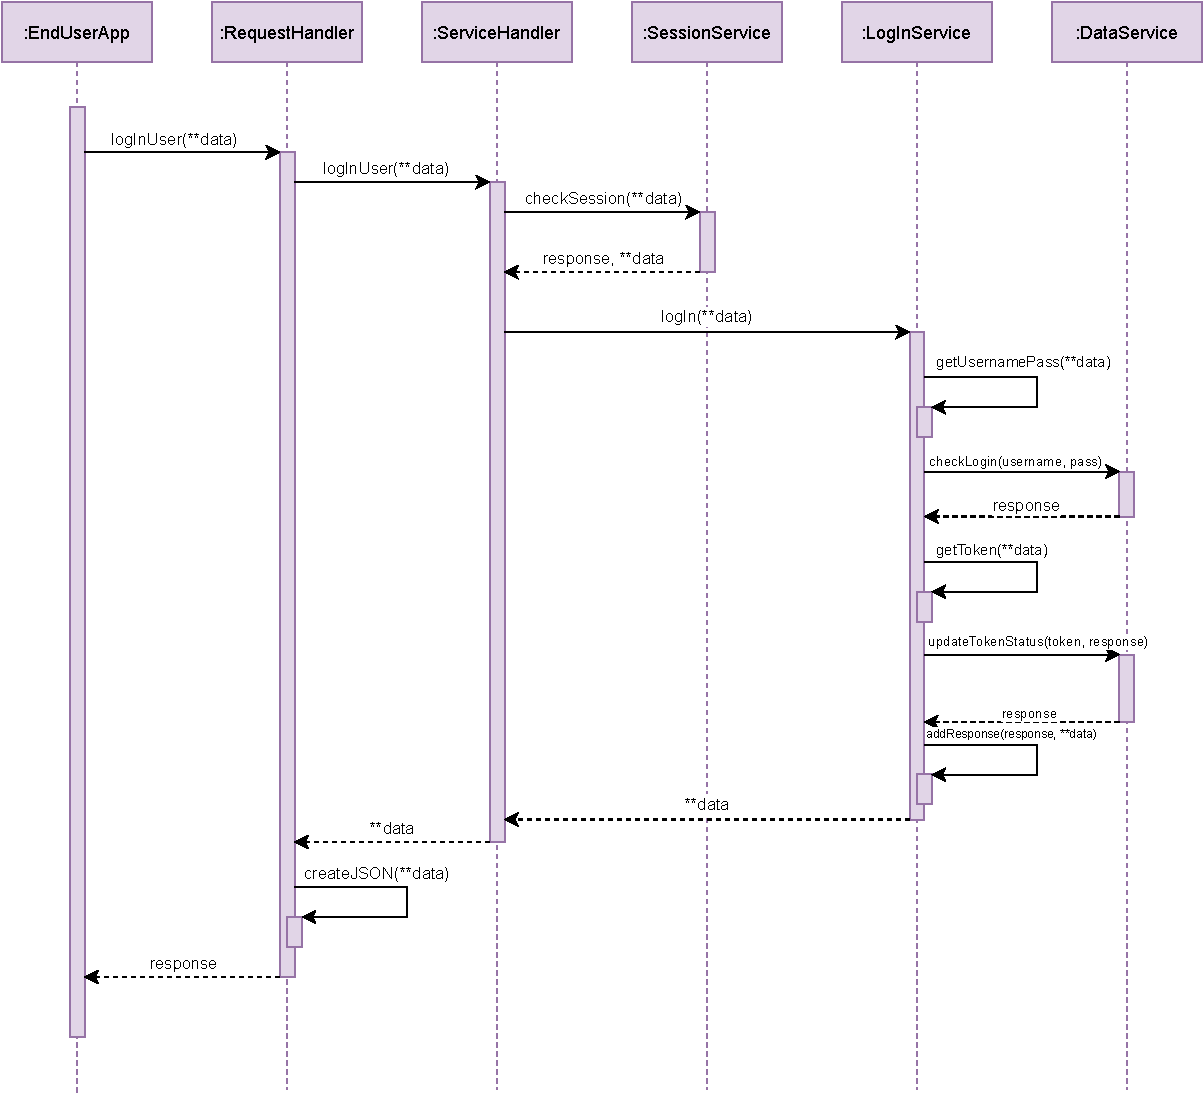
\includegraphics[width=1.0\textwidth]{images/logIn_sequence_diagram.pdf}
	\caption{Log In sequence diagram.}\label{fig:LogIn}
\end{figure}

\subsection{Lining Up}

In figure~\ref{fig:LiningUp} the lining up operation has been reported.
The user, to be allowed to perform a lining up, has to be registered and authenticated, therefore the ServiceHandler checks the token validity, communicating with the SessionService, and controls if the user is authenticated by getting the status of the token from the DataService.
In case of valid token with positive status (user before logged in), the request is forwarded to the LiningUpService, which after few controls, can decide to pass the lining up information to the Scheduler.
In any case the RequestHandler will reply to the clients with a response that it will contain lining up information (such as the QR code) or an error message.

\begin{figure}[H]
	\centering
	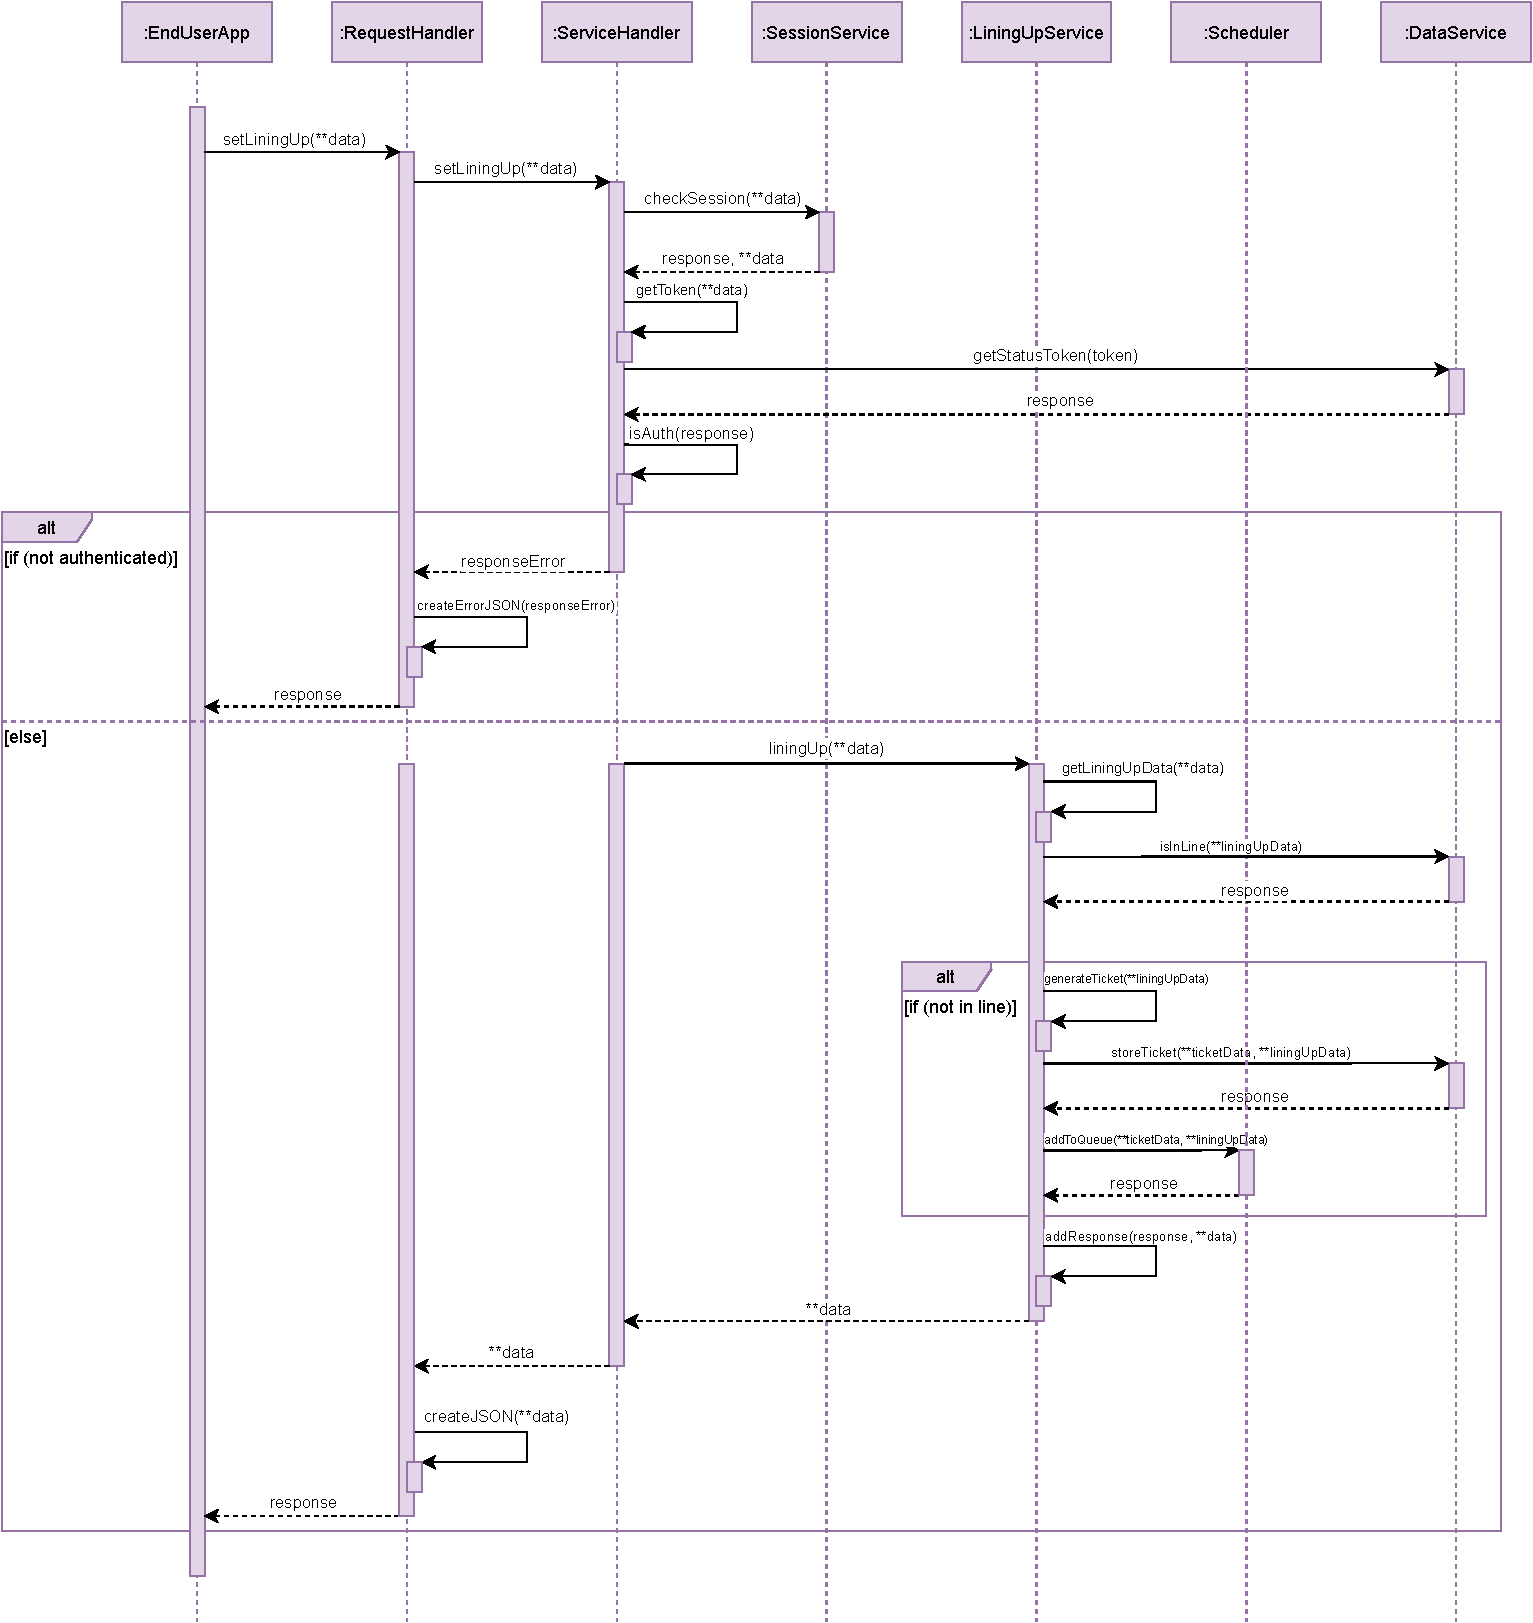
\includegraphics[width=1.0\textwidth]{images/liningUp_sequence_diagram.pdf}
	\caption{Lining Up sequence diagram.}\label{fig:LiningUp}
\end{figure}

\subsection{Booking a Visit}

The sequence diagram~\ref{fig:BookingVisit} is similar to the previous one.
The differences are in the kind of information passed from the EndUserApp.

\begin{figure}[H]
	\centering
	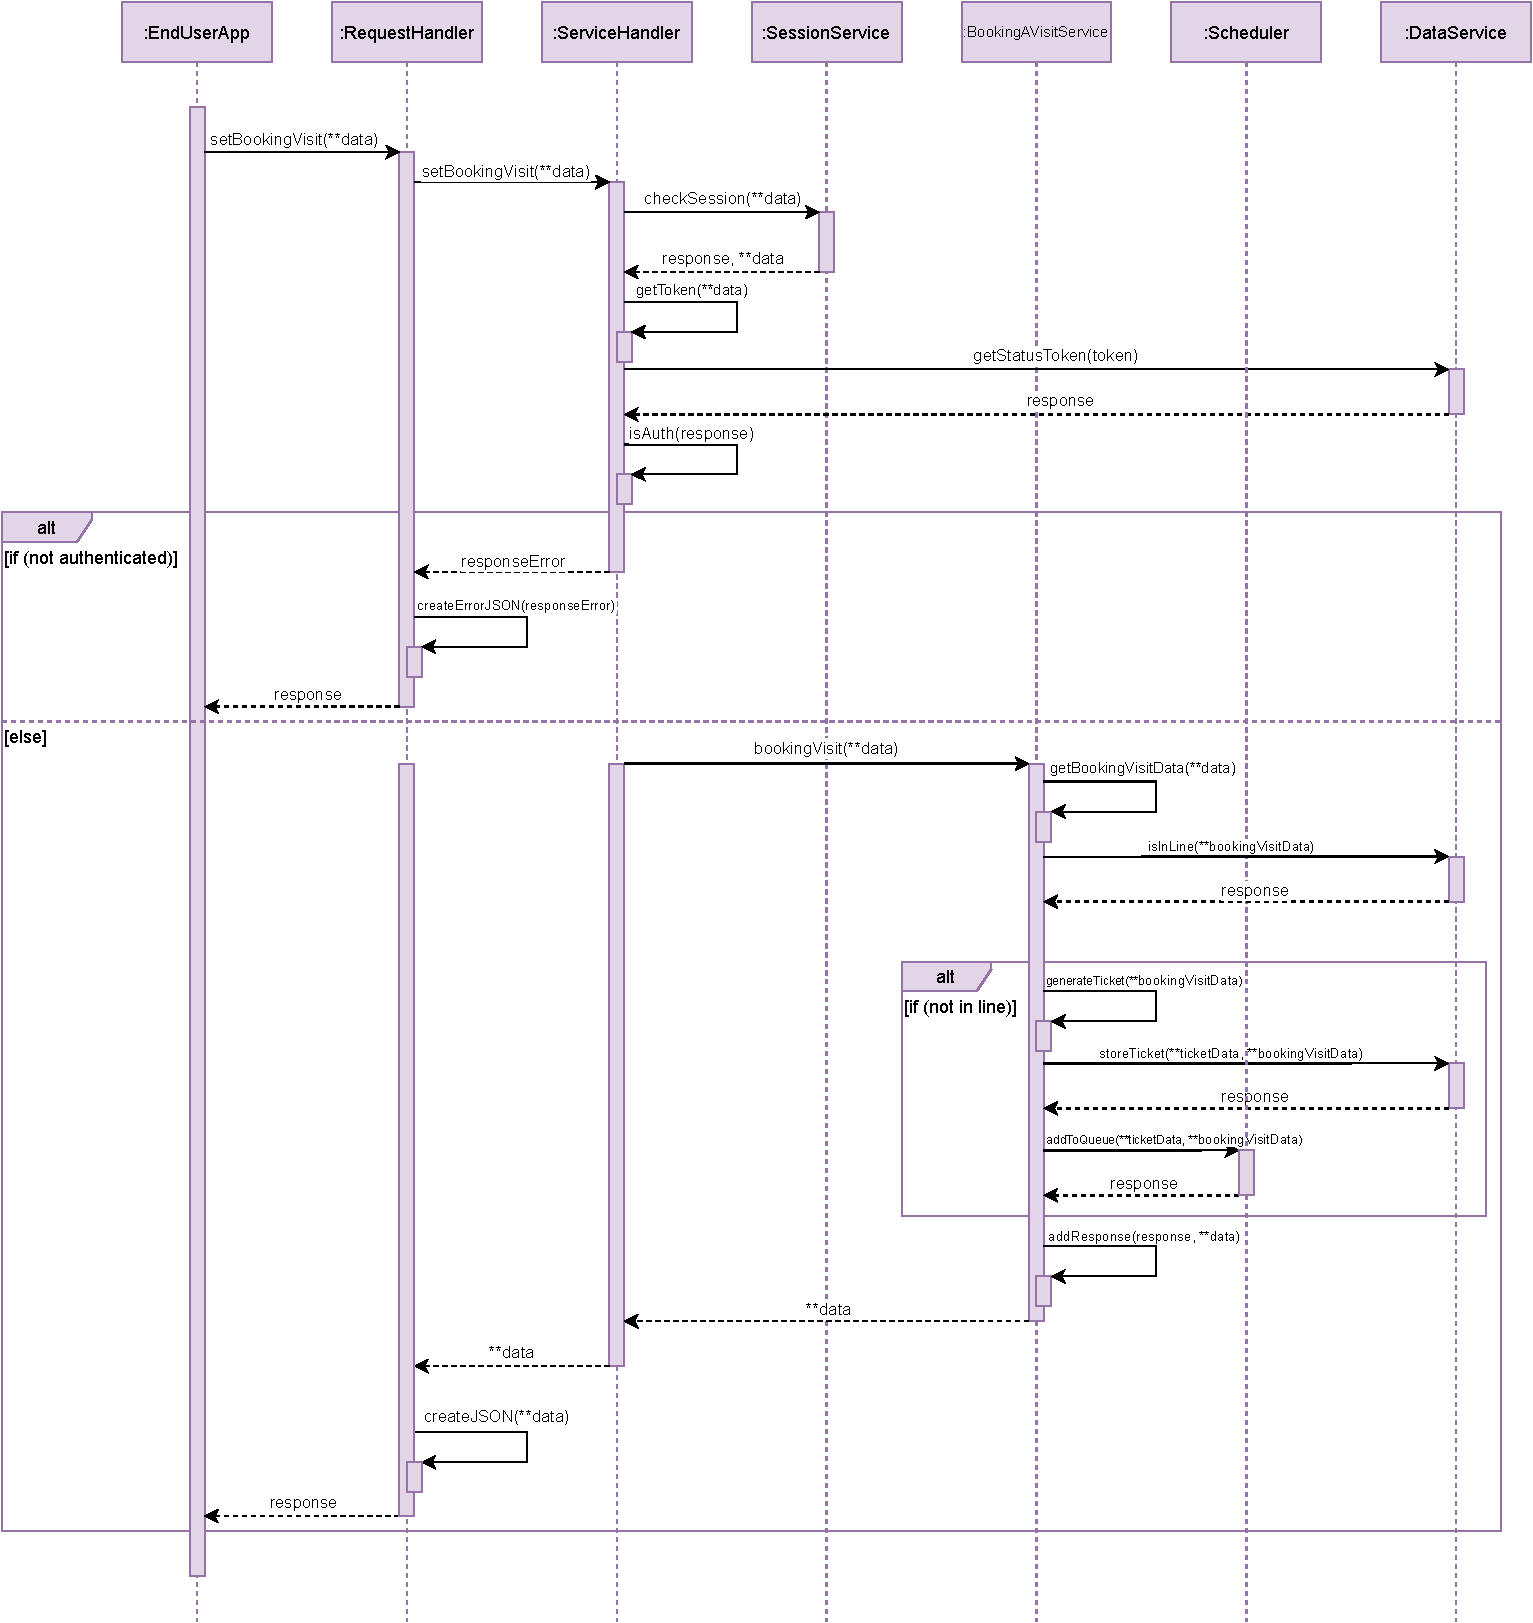
\includegraphics[width=1.0\textwidth]{images/bookingVisit_sequence_diagram.pdf}
	\caption{Booking a Visit sequence diagram.}\label{fig:BookingVisit}
\end{figure}

\subsection{Static Scheduler}

Figure~\ref{fig:StaticScheduler} illustrates the sequence of events that occur in the Scheduler after that the LiningUpService, or BookingAVisitService, has been activated.
It is called \textit{static} since these operations are performed only one time.
The main purpose of this sequence is to show how the system allocates tickets in the virtual queue. It estimates the time in which customers will be called by collecting data from the history of purchases of customers (GroceryStoreService) and the needed time to arrive to the store (GoogleMapsService). Once an estimation is computed, the allocation in the queue is determined.

\begin{figure}[H]
	\centering
	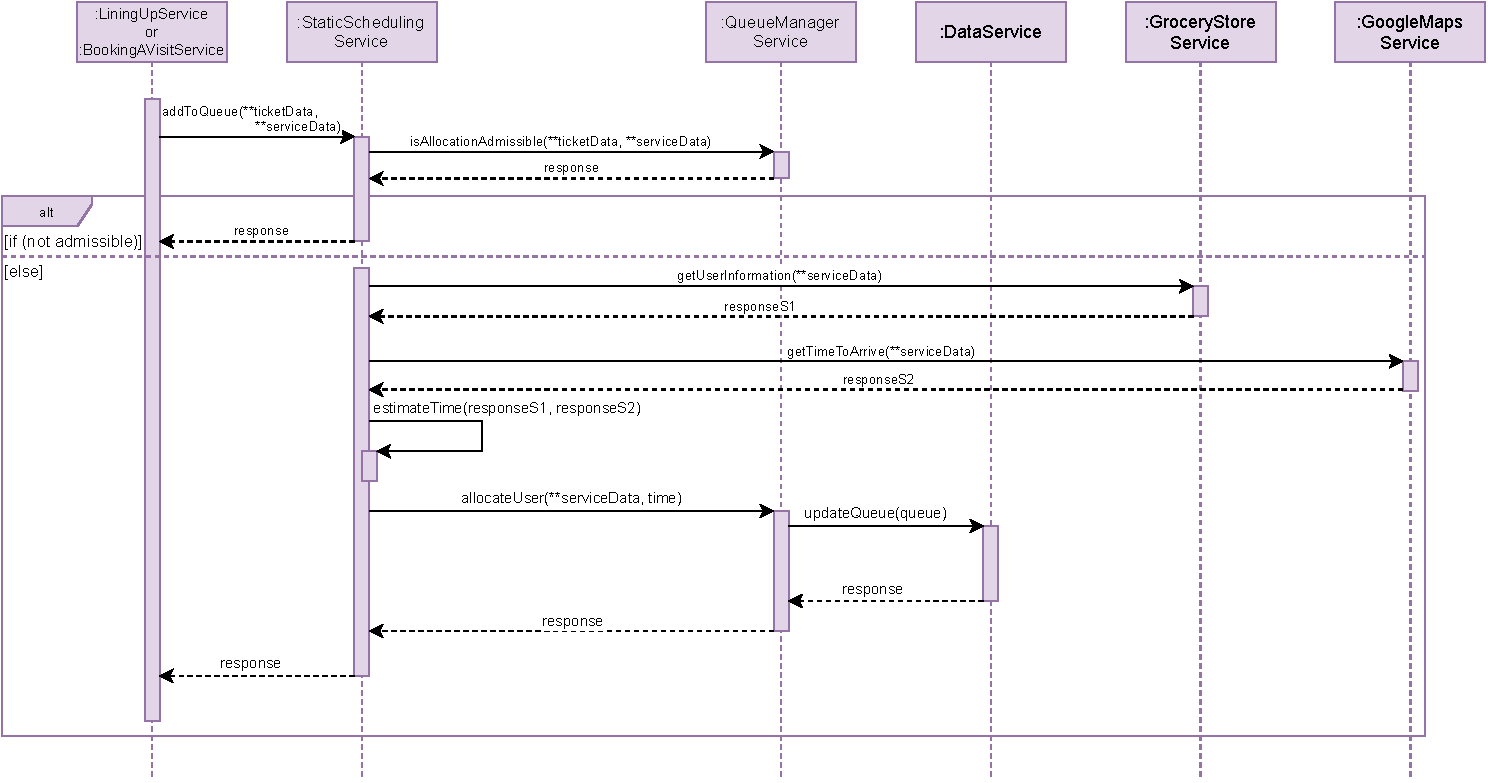
\includegraphics[width=1.0\textwidth]{images/scheduler_sequence_diagram.pdf}
	\caption{Static Scheduler sequence diagram.}\label{fig:StaticScheduler}
\end{figure}

\subsection{Dynamic Scheduler}

In contrast to the previous paragraph, in figure~\ref{fig:DynamicScheduler} there are activities that are performed mainly in background by the system to reschedule the virtual queue and to notify customers; for this reason it is called \textit{dynamic}.
The EndUserApp periodically sends information to the server about the location of the customers (in case of active tickets). These kind of requests are forwarded to the UserPositionService through the LiningUpService, or the BookingAVisitService. The UserPositionService is used to estimate the position of the customers and to update the queue through the QueueManagerService.
The QueueManagerService checks if it should notify users about timing and delays, moreover it updates the queue if tickets are expired.

\begin{figure}[H]
	\centering
	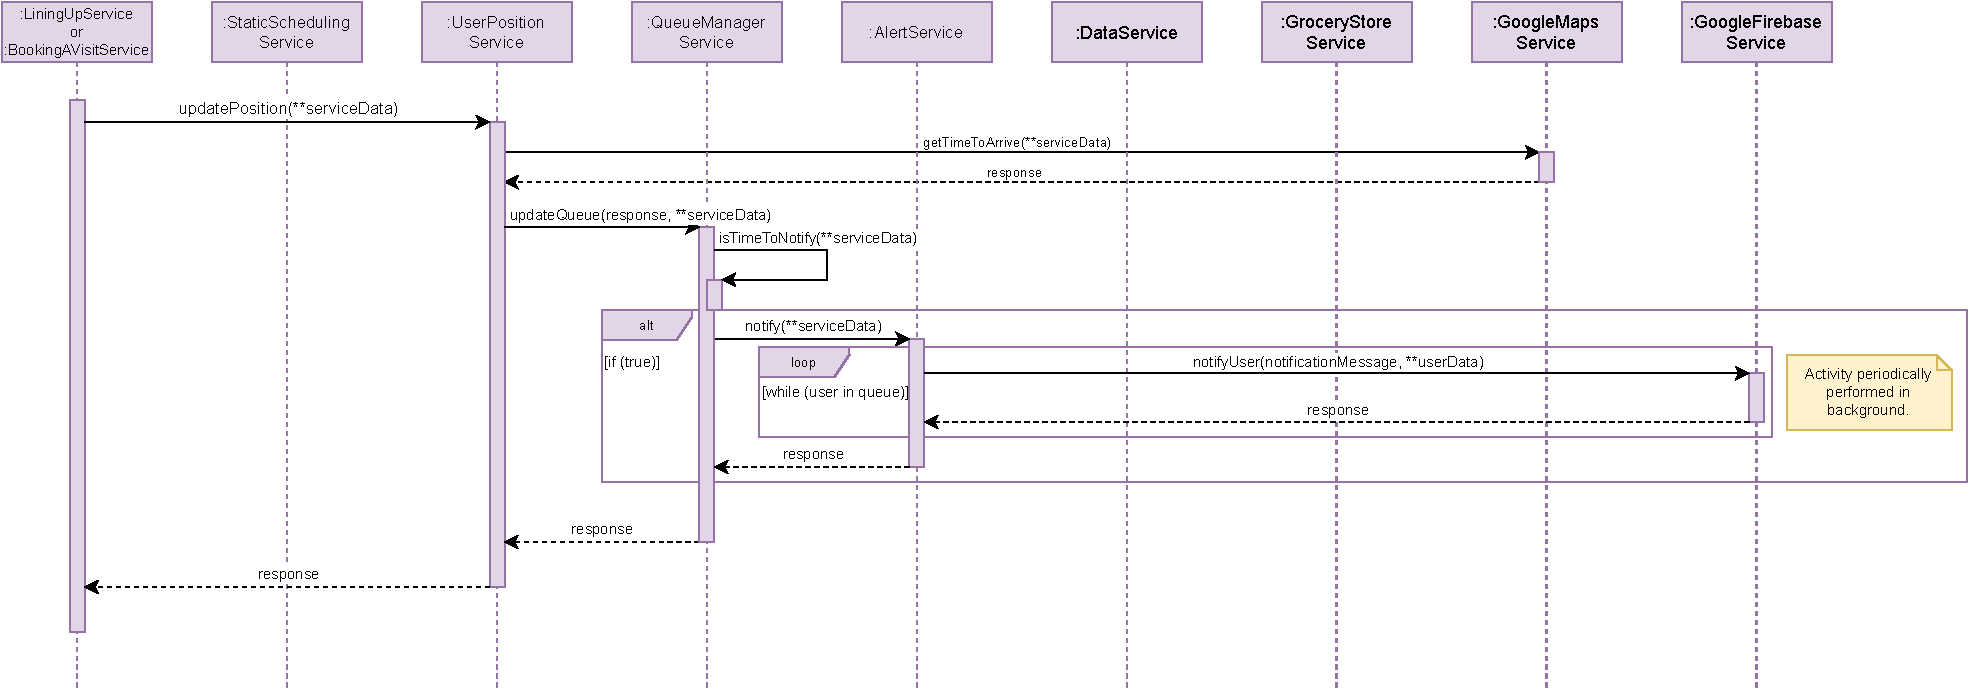
\includegraphics[width=1.0\textwidth]{images/dynamicScheduler_sequence_diagram.pdf}
	\caption{Dynamic Scheduler sequence diagram.}\label{fig:DynamicScheduler}
\end{figure}

\subsection{Control Queue}

\begin{figure}[H]
	\centering
	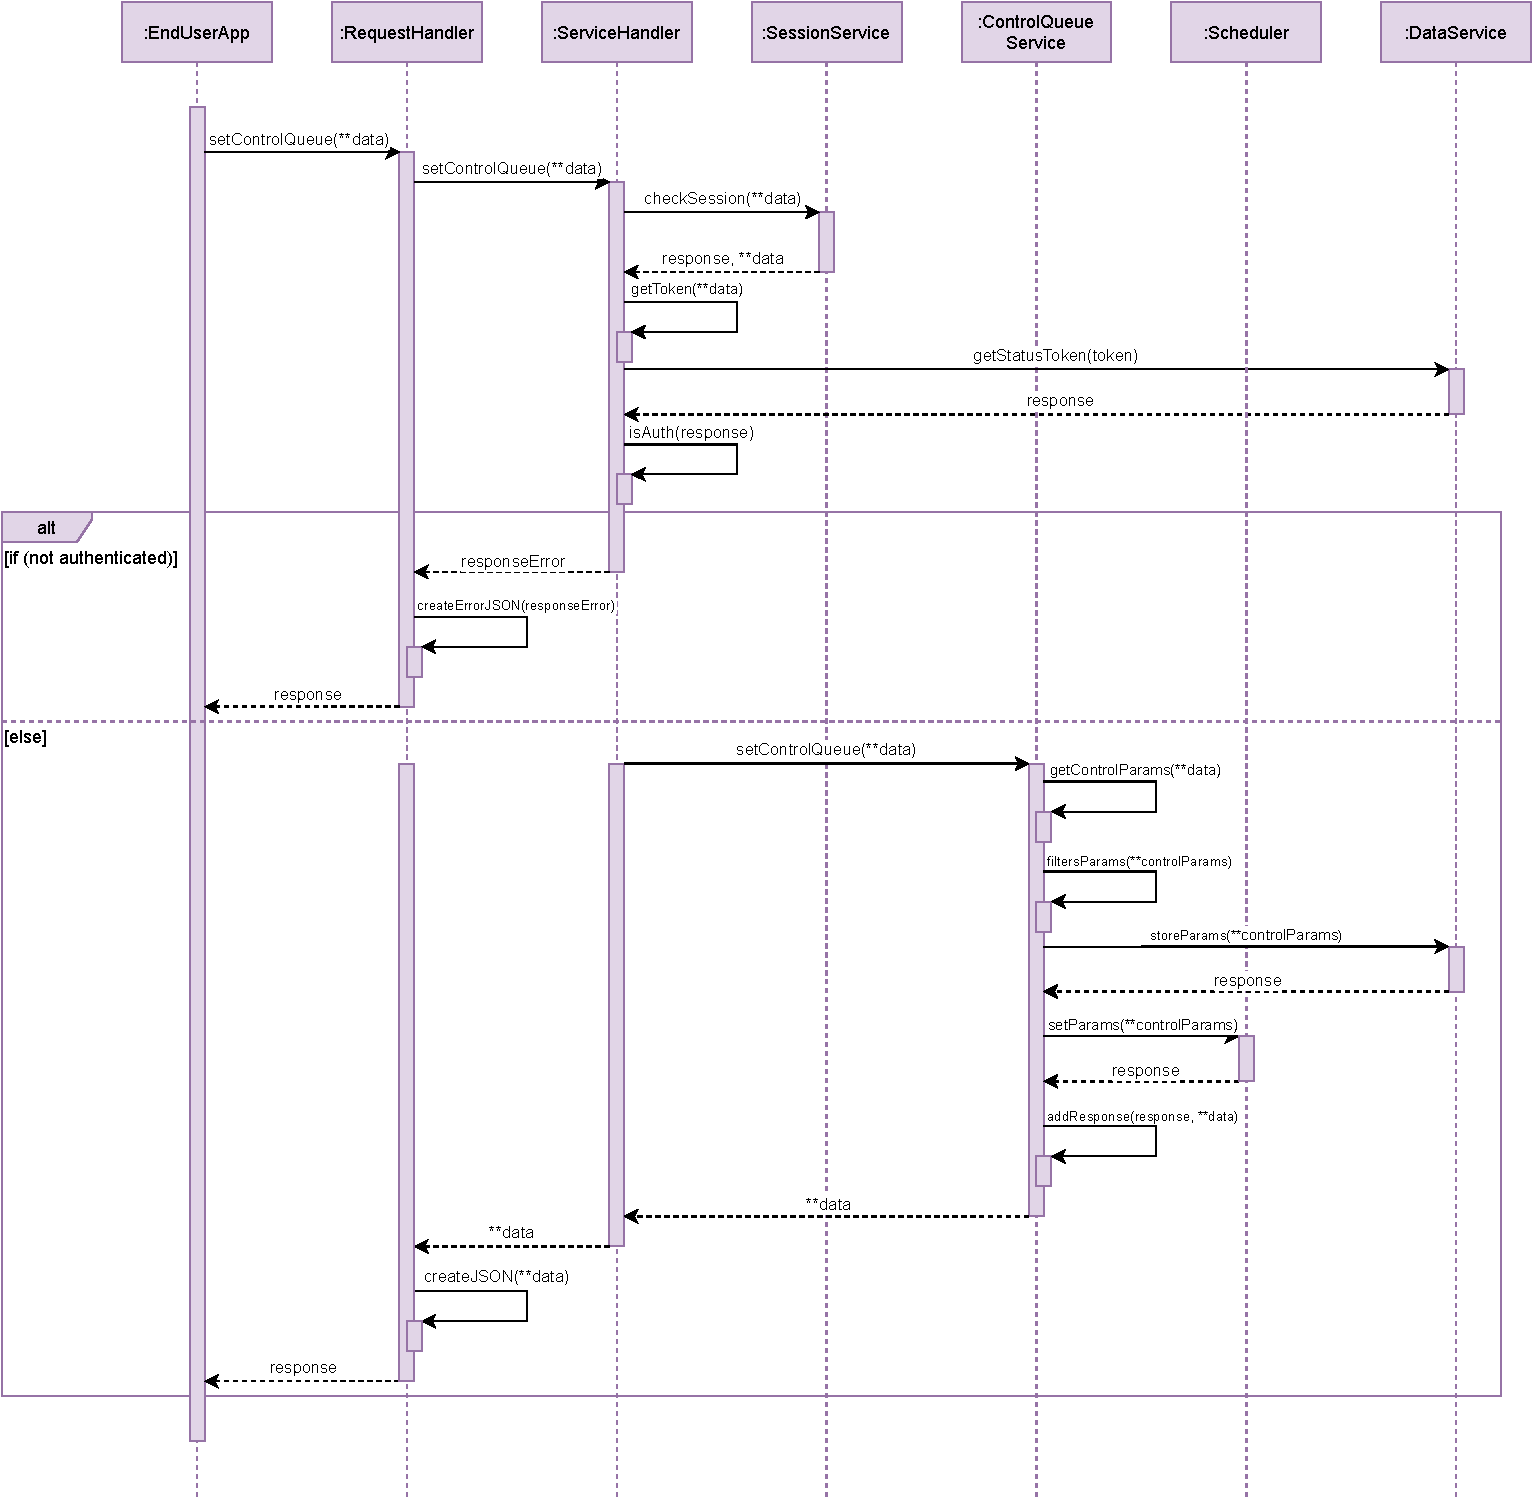
\includegraphics[width=1.0\textwidth]{images/controlQueue_sequence_diagram.pdf}
	\caption{Control Queue sequence diagram.}
\end{figure}

\begin{figure}[H]
	\centering
	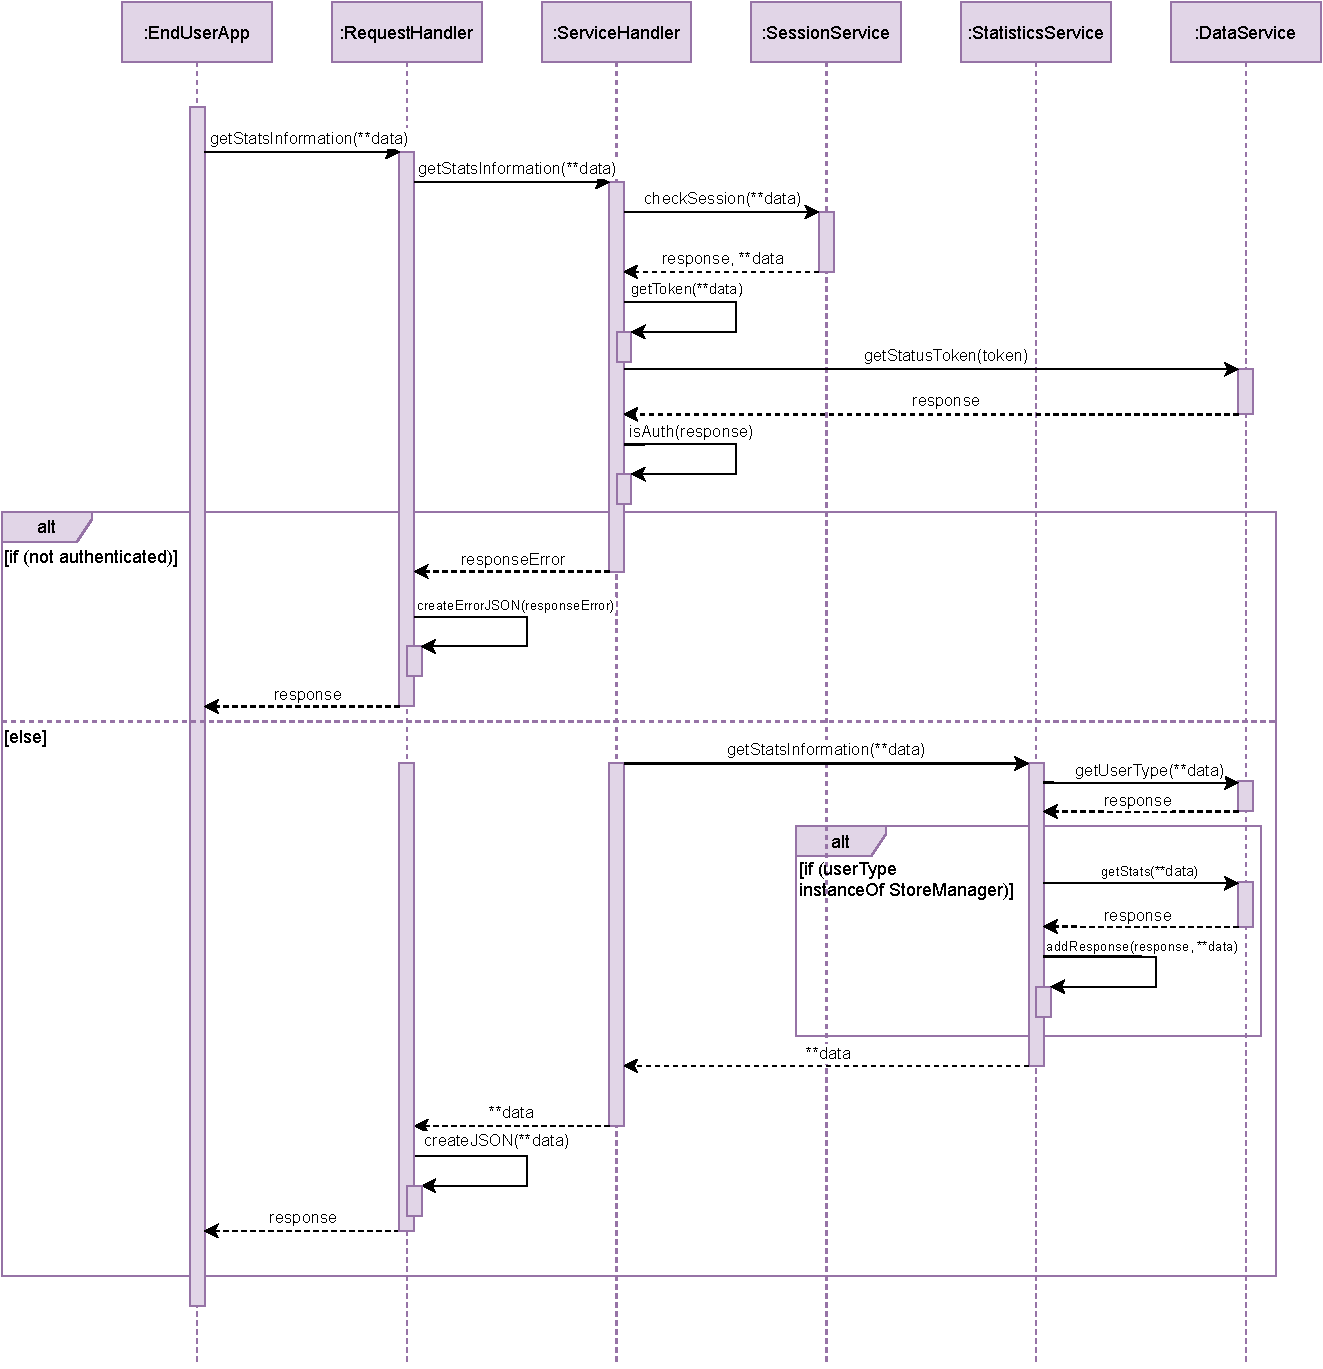
\includegraphics[width=1.0\textwidth]{images/showStats_sequence_diagram.pdf}
	\caption{Show Stats sequence diagram.}
\end{figure}

\begin{figure}[H]
	\centering
	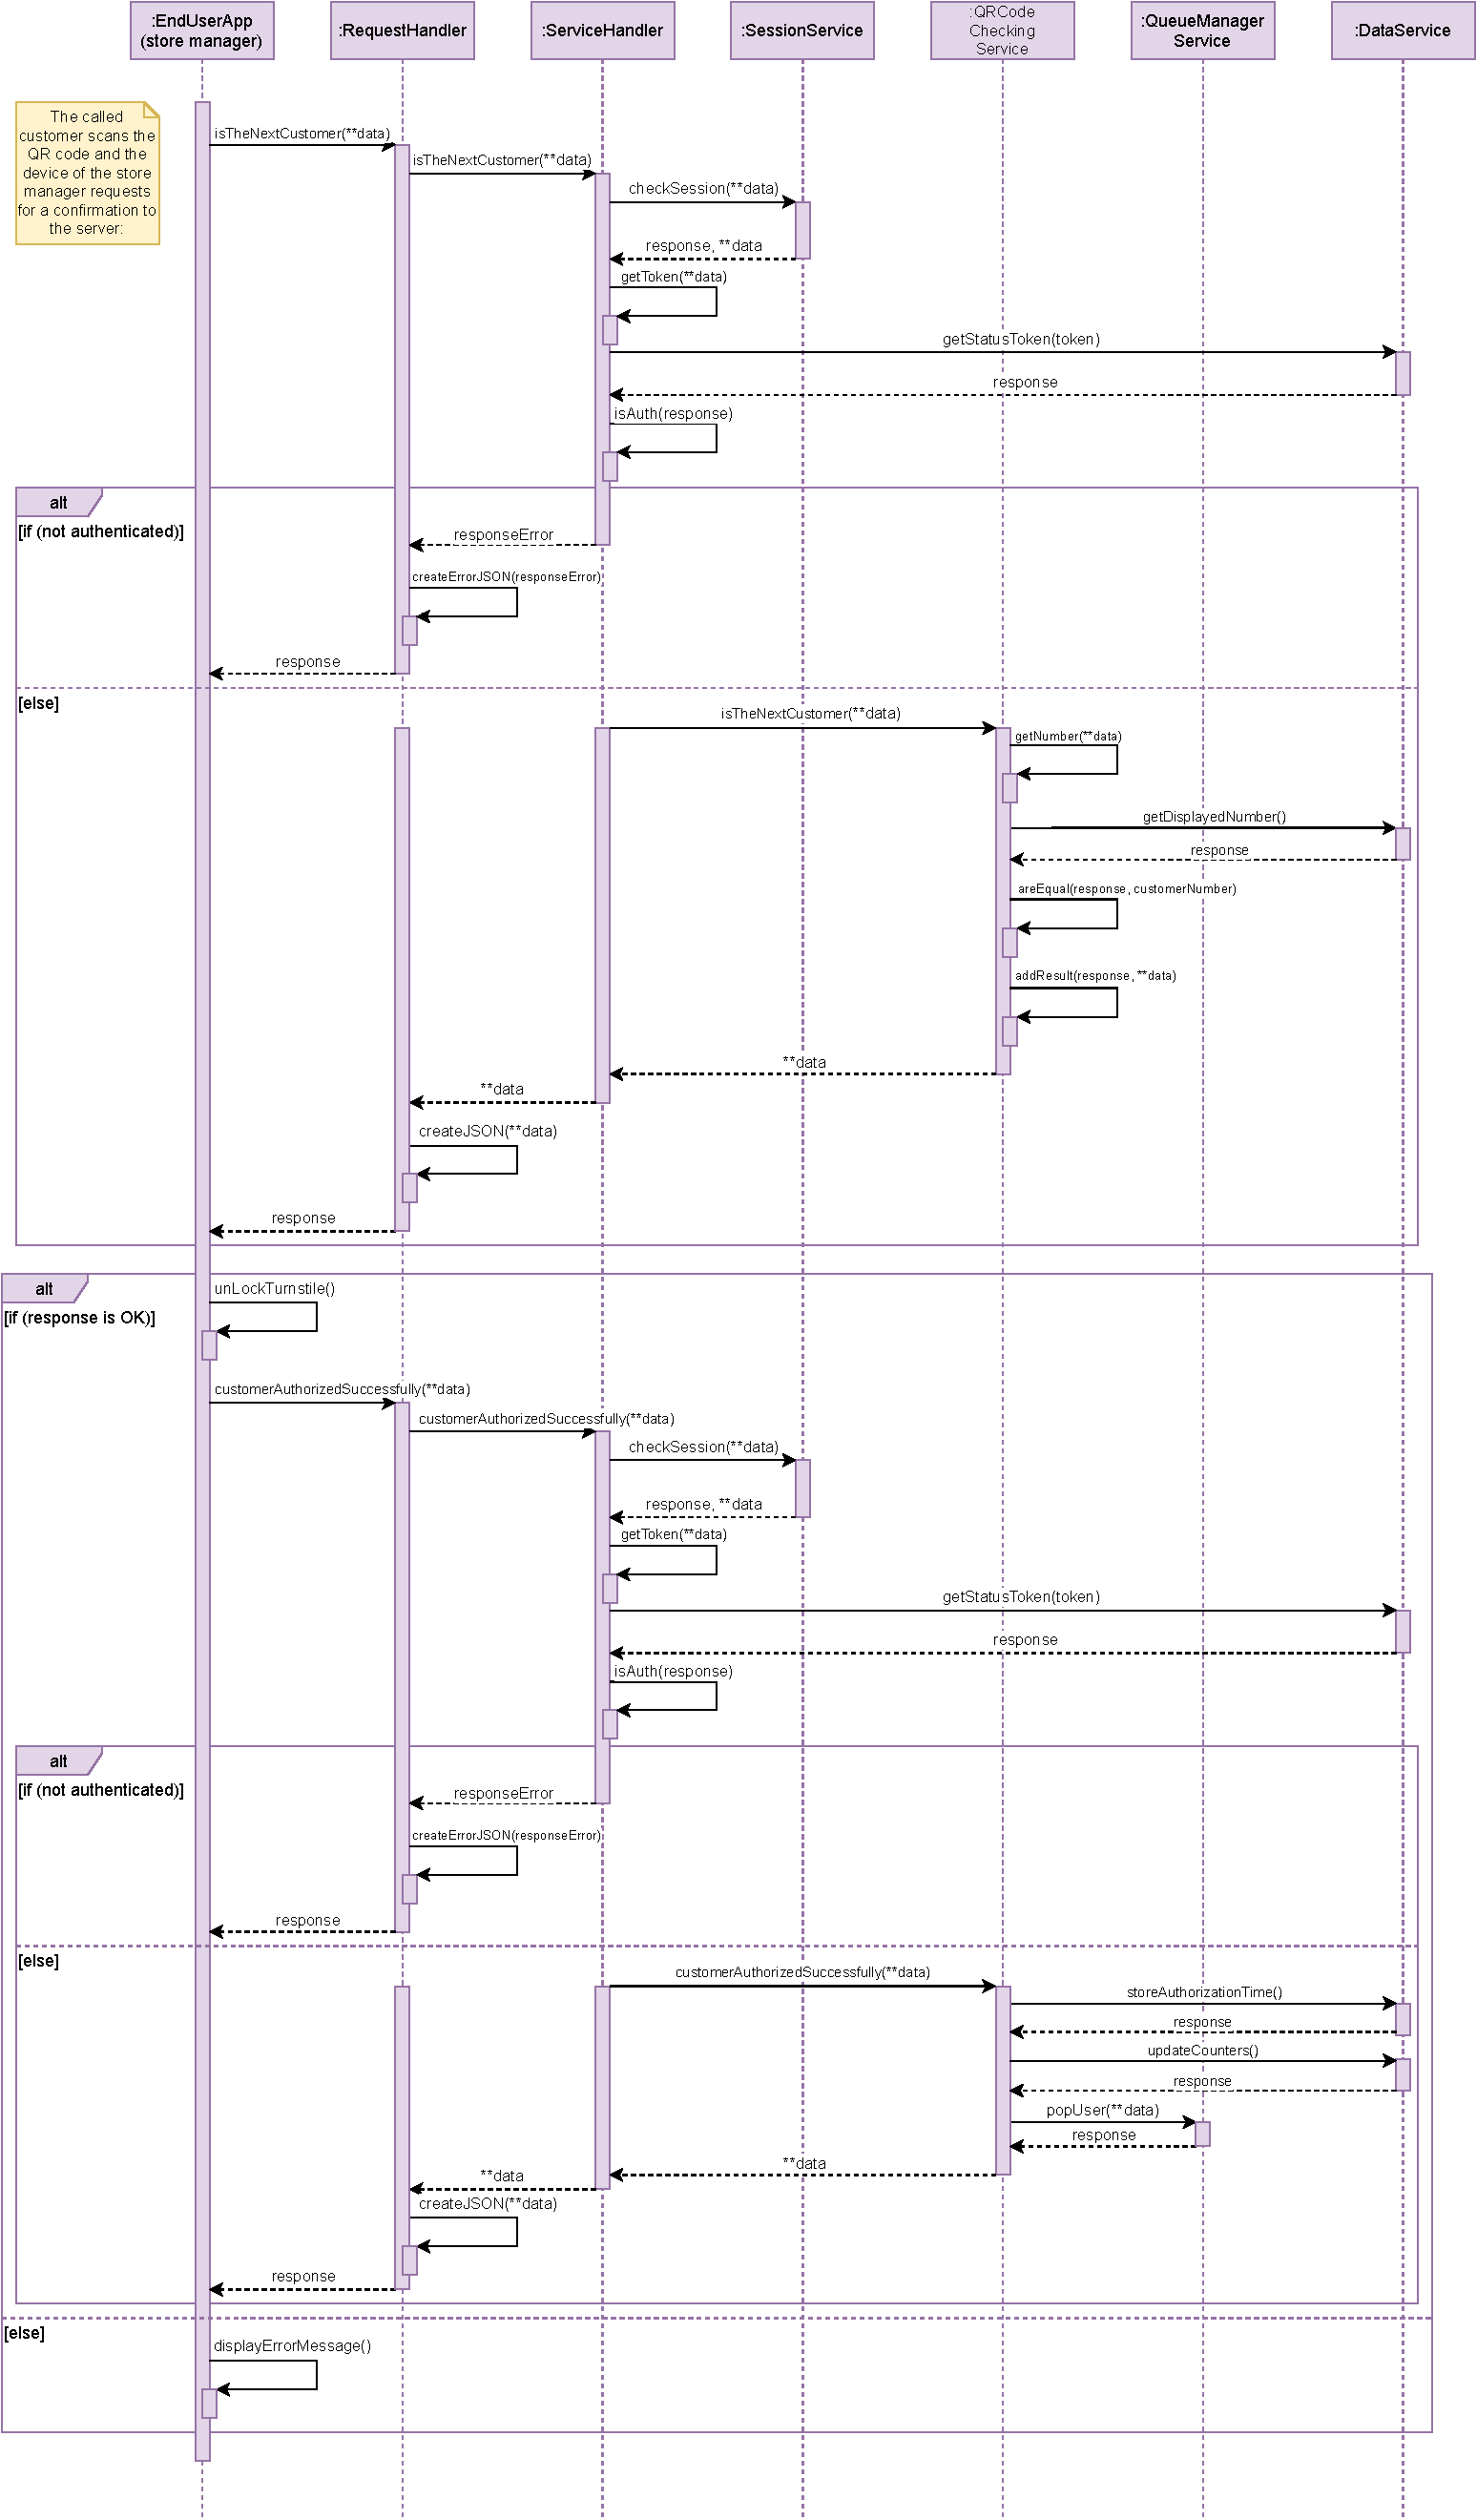
\includegraphics[width=0.8\textwidth]{images/qrCodeChecking_sequence_diagram.pdf}
	\caption{QR Code Checking sequence diagram.}
\end{figure}

\section{Component Interfaces}

\section{Selected Architectural Styles and Patterns}

\begin{figure}[H] % \begin{sidewaysfigure}
	\centering
	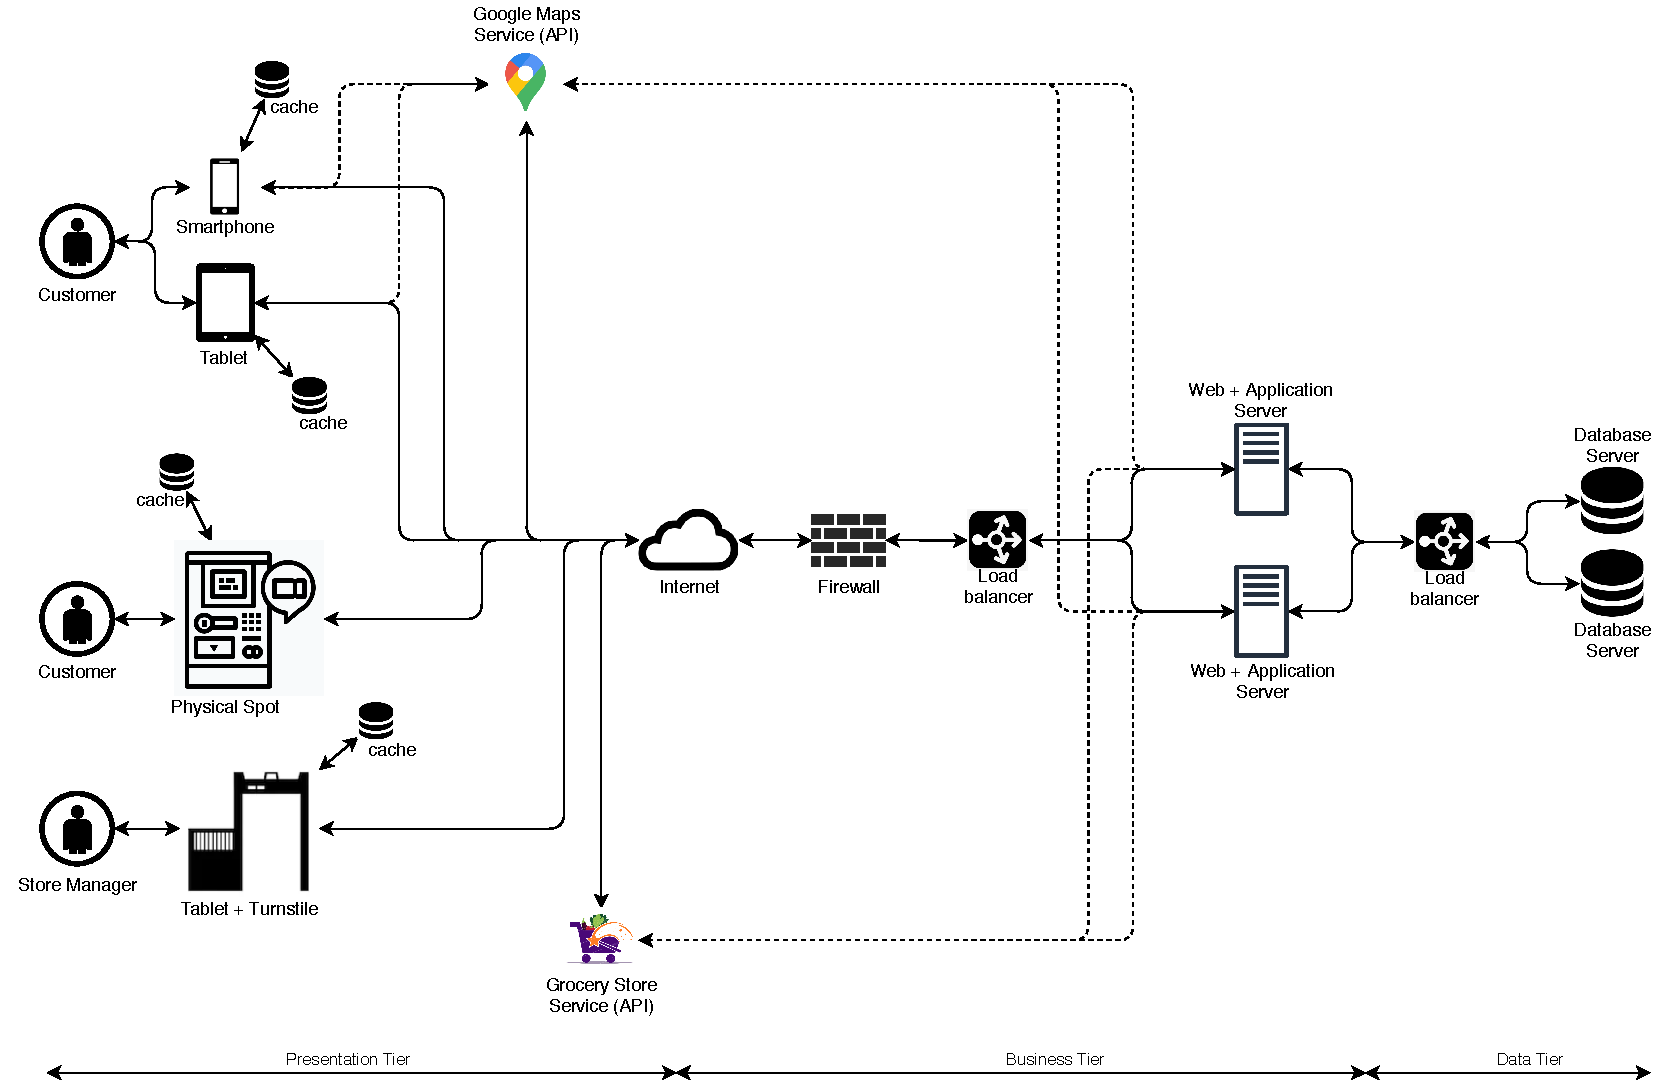
\includegraphics[width=1.0\textwidth]{images/architecture_components.pdf}
	\caption{Architecture components.}
\end{figure} % \end{sidewaysfigure}

\section{Other Design Decisions}